\chapter*{General introduction}
\markboth{General introduction}{}
\addstarredchapter{General introduction}

% > Microphysics in (P)NS (nuc)
%   > EoS (core)
%     > NN interaction (Skyrme, RMF - DFT, ab initio)
%     > SNA
%     > NSE
%   > TOV
%
% > Organization of the thesis

\section*{Astrophysical context}

% hyp ns
The existence of dense stars was hypothesized as early as 1931 
by Landau~\cite{Landau1932}, a year before the discovery of neutrons by
Chadwick~\cite{Chadwick1932}. 
Landau anticipated that the stellar matter density may become ``so great that 
atomic nuclei come in close contact, forming one gigantic 
nucleus''. 
% formation via sn
In 1934, Baade and Zwicky introduced the term \textit{supernova} (SN) to 
designate a ``remarkable type of giant novae'', a rare and very energetic 
phenomenon, characterized by a sudden and ephemeral burst in luminosity 
followed by a slow decay, and they predicted that ``supernovae represent the 
transitions from ordinary stars to \textit{neutron stars}''~\cite{Baade1934}.
% discovery
The presence of neutron stars (NS) in the Universe remained purely theoretical 
until 1968, when a rapidly pulsating source, a \textit{pulsar}, was observed 
for the first time by Jocelyn Bell, a graduate student supervised by 
Hewish~\cite{Hewish1968}. Several weeks after this observation, and motivated 
by the discovery of the Crab pulsar in 1968 which could not be identified as a 
white dwarf on account of a very short pulsation period~\cite{Comella1969}, 
pulsars were identified as ``rotating neutron stars'' by Gold~\cite{Gold1968}, 
paving the way for important theoretical development and observations in the 
following decades.

% sn
Given the available historical records of SN occuring in the Milky Way over the
past two thousand years~\cite{Green2003}, the SN rate in our galaxy is 
estimated to be quite low. Indeed, only five or six galactic SN have been 
recorded since 1000 CE, and only extragalactic SN have been observed for a 
century~\cite{Bergh1991}, notably the famous SN 1987A occuring in 1987 in the 
Large Magellanic Cloud, which is the most well-observed SN explosion to date.
% classifications
SN have been classified into different types, depending on their 
spectroscopic properties. 
Type I SN display no hydrogen lines, but show $^{56}$Fe as well as $^{56}$Co
lines. Conversely, type II SN exhibit strong Balmer lines, which is the sign of
an expanding atmosphere.
%
For the type Ia showing a lack of hydrogen lines but strong silicon absorption 
lines, it is commonly accepted that they result from thermonuclear explosion of 
white dwarfs, leaving no compact remnant.
In the consensus view, the other explosion types are triggered by the core 
collapse of massive stars, eventually leading to the formation of a NS or a 
black hole. 
It should be noticed that NS can also originate from accretion induced 
collapse, though the fraction of NS formed in this way is expected to be 
small~\cite{Fryer1999}.

% plan
In the following, we give a brief overview of the current understanding of the 
dynamics of core collapse supernovae (CCSN), and describe the transition from 
warm protoneutron stars (PNS) to NS. Measurements of NS observables, providing 
important constraints for dense matter properties, are also discussed.

\subsection*{Core collapse supernova}

% stellar evolution
The first stage of the active life of a star, generally referred to as main
sequence, consists in burning the hydrogen present in its core into helium,
and last until $\sim 90\%$ of the total mass is converted. Once this point is
reached, the inert helium core contracts under gravitational force.
% 
Depending on the mass of the star, the sequence of thermonuclear burning stage
is different. The maximum temperatures encountered in the center of subsolar 
mass stars are not high enough to burn helium into carbon, thus they cool down 
and become white dwarfs. 
More massive stars, $M \gtrsim 4-8M_\odot$ ($M_\odot$ being the solar mass), 
can proceed to the ignition of
helium into carbon, and then into oxygen, and they will ultimately turn into 
red giants. This will be the case for the Sun in approximately 5.4 billion 
years, when it will exit the main sequence.
The most massive stars, $M \gtrsim 8M_\odot$ can ignite their core elements up 
to silicon burning into iron ($T \sim 10^9$ K), then the fusion of elements is 
no longer possible because iron is the most stable nucleus. The chain of 
reactions in their core ends, and in their final stage the stars exhibit a 
onion-like structure, their core being composed of iron and neutron-rich 
iron-group nuclei~\cite{Bethe1979}, surrounded by shells of lower and lower 
burning elements (Si, O, C, He, H) up to possible inert hydrogen, at 
progressively lower temperatures and densities~\cite{Woosley2002}. 
Such stars are called presupernova or progenitor of CCSN. 
%
At this point, the inert core is essentially sustained by the electron
degeneracy pressure. 
The mass of the iron core increases by silicon shell burning, and ultimately a 
critical mass limit is reached when the gravitional force overcomes the 
degeneracy pressure, leading to the contraction of the core. 
This limit corresponds to the so-called Chandrasekhar 
mass~\cite{Chandrasekhar1931},
%
\begin{equation}
  M_{Ch} = 1.457(2Y_e)^2 M_\odot,
\end{equation}
%
where $Y_e$ represents the electron fraction. Let us note that a temperature
dependent corrections entering the expression of the Chandrasekhar mass have 
been proposed in the literature~\cite{Woosley2002}. 
According to the model calculations of stellar evolution which give similar 
final states of the core, characterized by a central density $\rho_c 
\sim 10^{10}$ g/cm$^3$, temperature $T_c \sim 10^{10}$ K, and entropy $s 
\sim k_B$ ($k_B$ being the Boltzmann constant), the electron fraction of the 
core is estimated to $Y_e \sim 0.42 - 46$, yielding a Chandrasekhar mass value 
of $M_{Ch} \sim 1.44 M_\odot$~\cite{Janka2007}.
%
When the mass of the iron core reaches the Chandrasekhar mass limit, it 
collapses under the overwhelming gravitational pressure, starting the CCSN. 
In the current picture, this process can be schematically divided into three 
stages, which we describe in what follows.

\begin{figure}[!t]
\begin{center}
  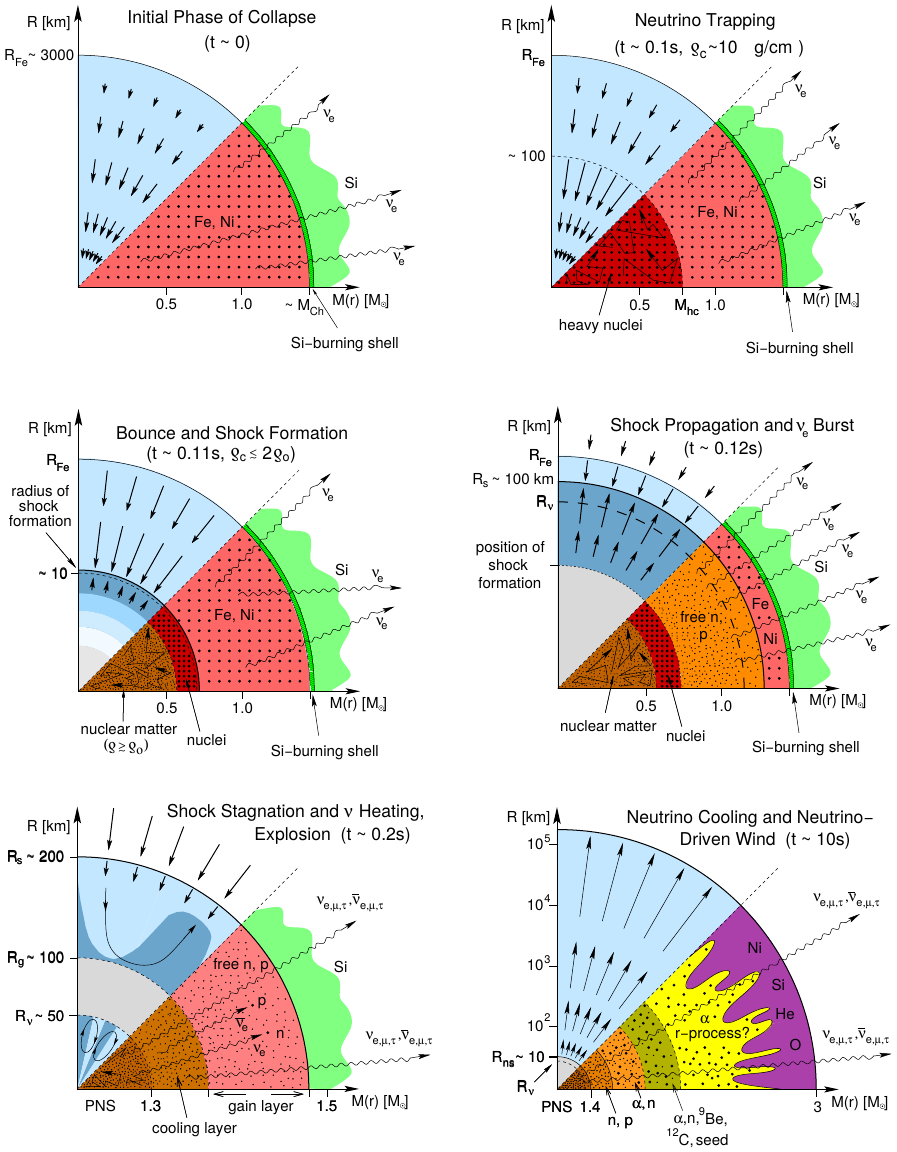
\includegraphics[width=0.965\linewidth]{figures/sn_intro.png}
\end{center}
\caption[Schematic representation of the evolutionary stages of a core collapse
supernova]{Schematic representation of the evolutionary stages of a CCSN.
  $M_{hc}$ corresponds to the homologous inner core mass, $M_{Ch}$ to the
  Chandrasekhar mass, and $R_{Fe}$, $R_s$, $R_g$, $R_{ns}$, and $R_\nu$ to the 
  iron core radius, shock radius, gain radius, neutron star radius, and 
  neutrinosphere, respectively. The arrows represent the velocity vectors. 
  Figure taken from~\cite{Janka2007}.}\label{fig:sn_intro}
\end{figure}
%
% infall phase
The infall epoch is characterized by the contraction of the iron core. 
In the initial phase of the collapse (upper-left panel of 
Fig.~\ref{fig:sn_intro}), the dynamics are very sensitive to the entropy and
electron fraction, which are mainly determined by weak interaction processes.
$Y_e$ decrases by electron capture in nuclei because of 
the increase in density and temperature. This has the effect of increasing 
the electron pressure with density, and consequently accelerating the infall 
mechanism and neutronizing the matter. Moreover, many of the neutron-nuclei 
undergo beta decay.
The endothermic reactions of partial photodisintegration of iron-group nuclei 
into alpha particles, and then of the alpha particles into neutrons and protons 
at higher tempreature, also accelerates the collapse. When the core density 
reaches $\rho_{trap} \sim 10^{12}$ g/cm$^3$, the medium is no longer
transparent to neutrinos. As a consequence, neutrinos are essentially trapped 
in the core because of the short collapse time with respect to their diffusion
time~\cite{Bethe1990}, and the beta equilibrium is established (upper-right 
panel of Fig.~\ref{fig:sn_intro}).
The infall is thus (quasi)adiabatic and the collapse is homologous,
which means that it behaves as a unit, collapsing self-similarly. 
The homologous inner core falls inward at subsonic velocity, while
the part of the iron core lying outside it, the outer core, falls at supersonic 
speed.

% bounce phase
The bounce phase is characterized by the formation of the shock wave, occuring 
only few hundred milliseconds after the beginning of the infall phase, when the 
density reaches approximately the saturation density, which corresponds to the 
equilibrium density of symmetric homogeneous infinite matter $\rho_{sat} \sim 
10^{14}$ g/cm$^3$. 
Due to the high incompressibility of nuclear matter, the internal pressure 
sharply counterbalances the gravitational effects and the collapse suddenly 
stops in propagating waves in the homologous core. However, the outer core 
continues to fall inwards at supersonic speed yielding an accumulation of the 
pressure waves at the sonic surface and finally driving a shock 
wave, characterized by a discontinuity in pressure and matter velocity 
(middle-left panel of Fig.~\ref{fig:sn_intro}). 
It is followed by the propagation of the shock wavethrough the rest of the iron 
core at supersonic velocity, eventually reaching the envelope of the star 
(middle-right panel of Fig.~\ref{fig:sn_intro}).

% explosive phase
The explosive phase is the final one, and corresponds to the propagation of
the shock wave and the expulsion of the outer layers, triggering the SN 
explosion that leaves a compact remnant at the center.  
Indeed, while in the scenario of the prompt mechamism the initial energy 
carried by shock wave could be sufficient to trigger the explosion, a 
considerable amount of energy is lost because of the photodissociation of iron 
core nuclei into neutrons and alpha particles, and neutrinos produced by 
electron capture leaving the star, once the neutrinosphere is reached by the 
shock wave (middle-right panel of Fig.~\ref{fig:sn_intro}). 
The weakened shock thus finally stalls at several hundred 
kilometers from the core, while matter behind the shock continues falling 
inwards, forming a PNS (lower-left panel of Fig.~\ref{fig:sn_intro}).
The comprehension of the mechanism triggering the explosion remains unclear,
and various propositions have been advanced in the literature, insisting of
different aspects such as hydrodynamic instabilities, rotation, g-mode 
oscillations, or magnetic field~\cite{Janka2007}.
%
In the delayed mechanism, the neutrinos streaming off the neutrinosphere carry 
most of the energy and can revive the shock wave by deposing some in the region
between the PNS and the stalled shock~\cite{Janka2007}.
The neutrino heating increases pressure behind the shock, expands the layers 
and creates a region of high temperature and low density, which by convection
allows the neutrino energy to be efficiently absorbed by the shock wave
(lower-left panel of Fig.~\ref{fig:sn_intro}). The high pressure 
could drive the shock further out and let it reach the envelope of the star, 
finally triggering the explosion (lower-right panel of 
Fig.~\ref{fig:sn_intro}), during which the outer layers of the star are 
ejected, enriching the stellar medium with the elements produced during the 
different burning stages, as well as during the supernova explosion, via $s$- 
and $r$-processes~\cite{Woosley2002,Janka2007}.

\subsection*{(Proto)neutron stars}

Blabla.

%  supernova remnant is a pns
%  pns will ultimately lead to a ns or a bh if its mass is larger than the NS
%   maximum mass corresponding to TOV limit, which is sensitive to the nuclear
%   EoS

%  cooling
%  crystallization

\begin{figure}[!t]
\begin{center}
  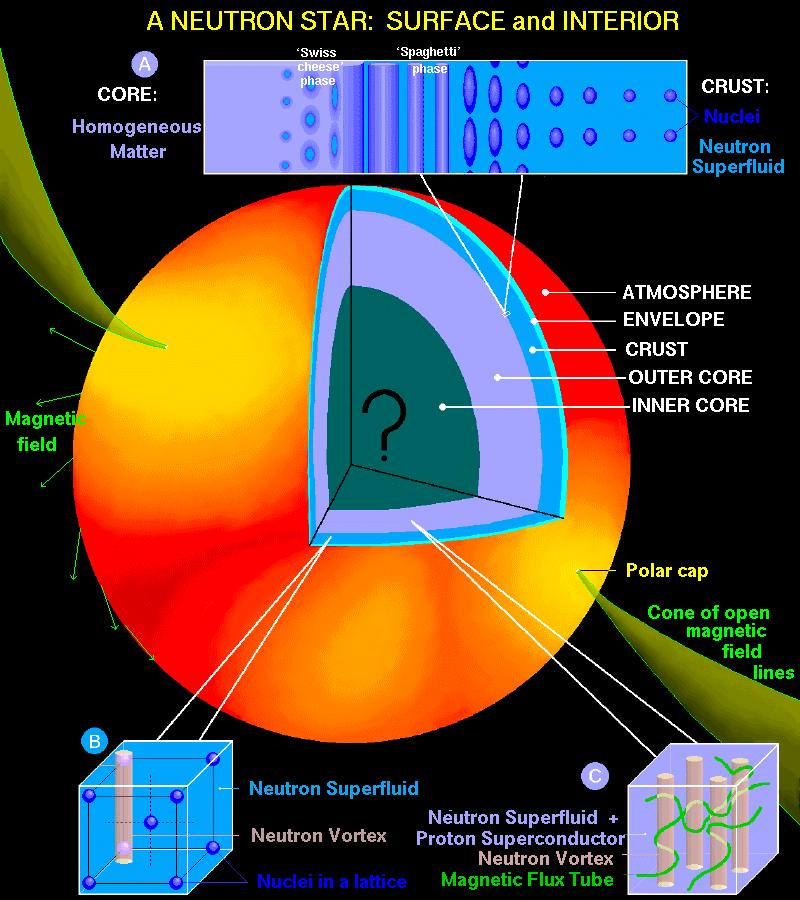
\includegraphics[width=0.8\linewidth]{figures/NStarInt.jpeg}
\end{center}
\caption[Schematic representation of the inside of a neutron star]{Schematic
representation of the inside of a NS. Figure taken 
from~\cite{Page2006}.}\label{fig:NStarInt}
\end{figure}
%
% describe structure NS

\subsection*{Observations}

% masses (only in binary)

% radius

% glitches

% gw

\section*{Microphysics of (proto)neutron stars}

\section*{Organization of the thesis}

\clearpage\thispagestyle{empty}
